\section{Empirical Scaling Experiments}

\paragraph{Experimental setup.}
The synthetic scaling experiments sample random digit supports and digit
amplitudes across bases \(B\in\{2,10,16\}\), digit lengths such as \(8\) and
\(16\) in the default reproducible grid, and support densities
\(\{0.2,0.5,0.7,1.0\}\). For each configuration, random pairs are generated
and passed through the projection--carry pipeline. The generated summary and
correlation tables are stored in the \texttt{paper/tables} directory.

\paragraph{Predictors and outcomes.}
The geometry predictors are sumset size, maximum representation count,
additive energy, support densities, and diagonal mass concentration. The carry
outcomes are carry mass, carry count, maximum carry cascade length, carry
amplification ratio, and normalized value-weighted carry. We also examine
normalized quantities such as carry mass per digit and cascade fraction.

\paragraph{Raw support concentration and carry mass.}
Figure~\ref{fig:additive-energy-carry-mass} shows additive energy against
carry mass. Additive energy measures concentration of representation counts on
anti-diagonals; high energy indicates that many support pairs may collide on a
small set of degrees. Figure~\ref{fig:max-rep-carry-mass} gives the related
view using the largest representation count. In the synthetic grid, both
quantities behave as structural predictors for absolute carry mass.

\begin{figure}[ht]
    \centering
    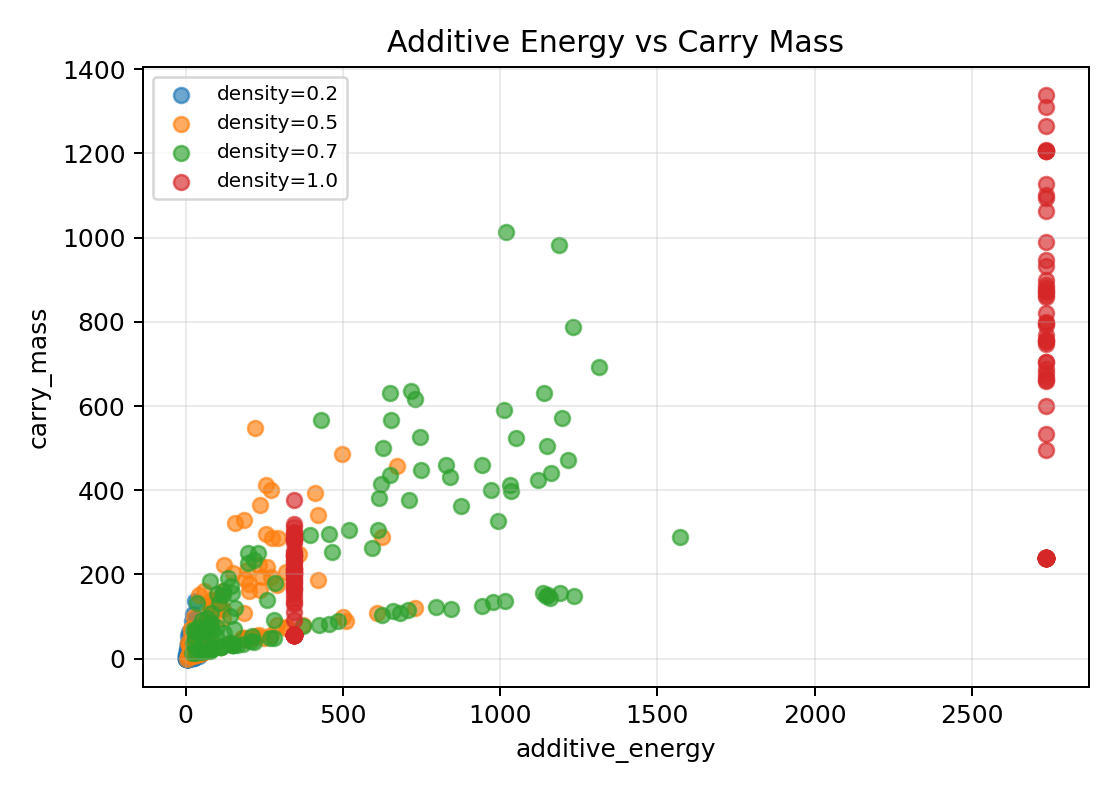
\includegraphics[width=0.78\linewidth]{figures/additive_energy_vs_carry_mass.png}
    \caption{Additive energy versus carry mass.}
    \label{fig:additive-energy-carry-mass}
\end{figure}

\begin{figure}[ht]
    \centering
    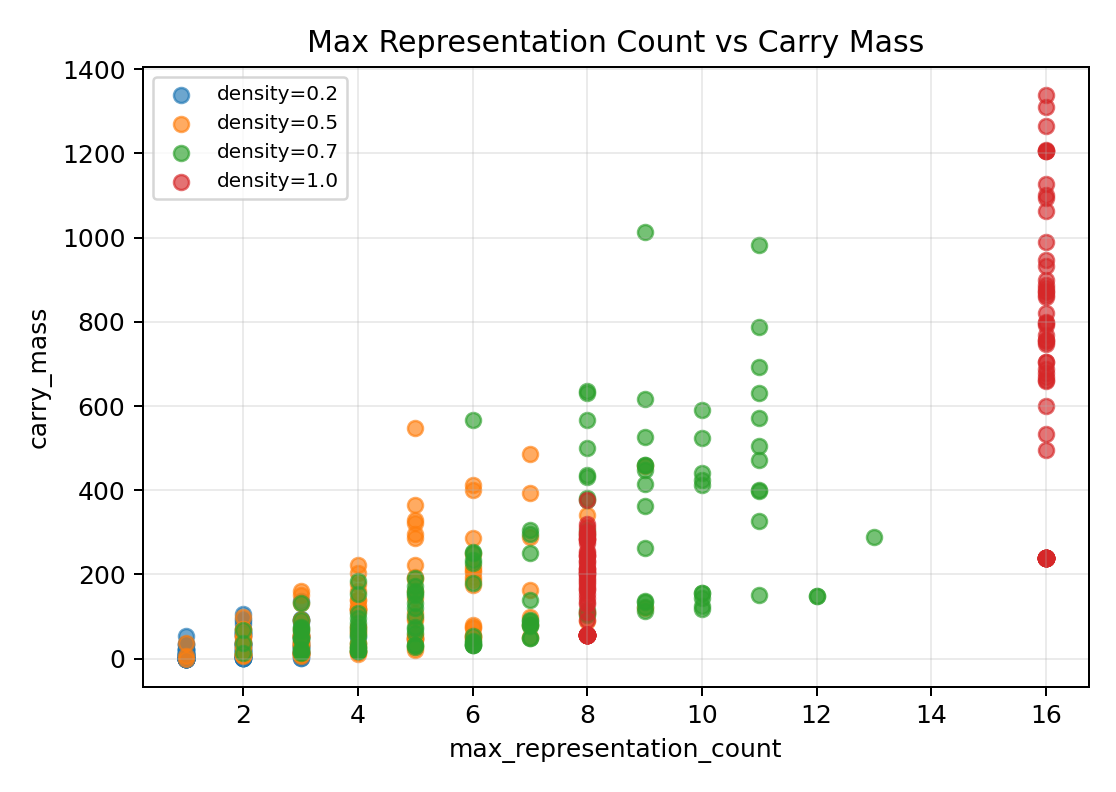
\includegraphics[width=0.78\linewidth]{figures/max_representation_vs_carry_mass.png}
    \caption{Maximum representation count versus carry mass.}
    \label{fig:max-rep-carry-mass}
\end{figure}

\paragraph{Spatial extent of carry flow.}
Figure~\ref{fig:sumset-carry-count} compares sumset size with carry count.
Sumset size tracks how many degree positions can receive raw mass; this is
therefore related to the spatial extent of carry activity. Figure~\ref{fig:density-cascade}
shows that support density is associated with cascade fraction, the normalized
length of the longest consecutive active-carry segment.

\begin{figure}[ht]
    \centering
    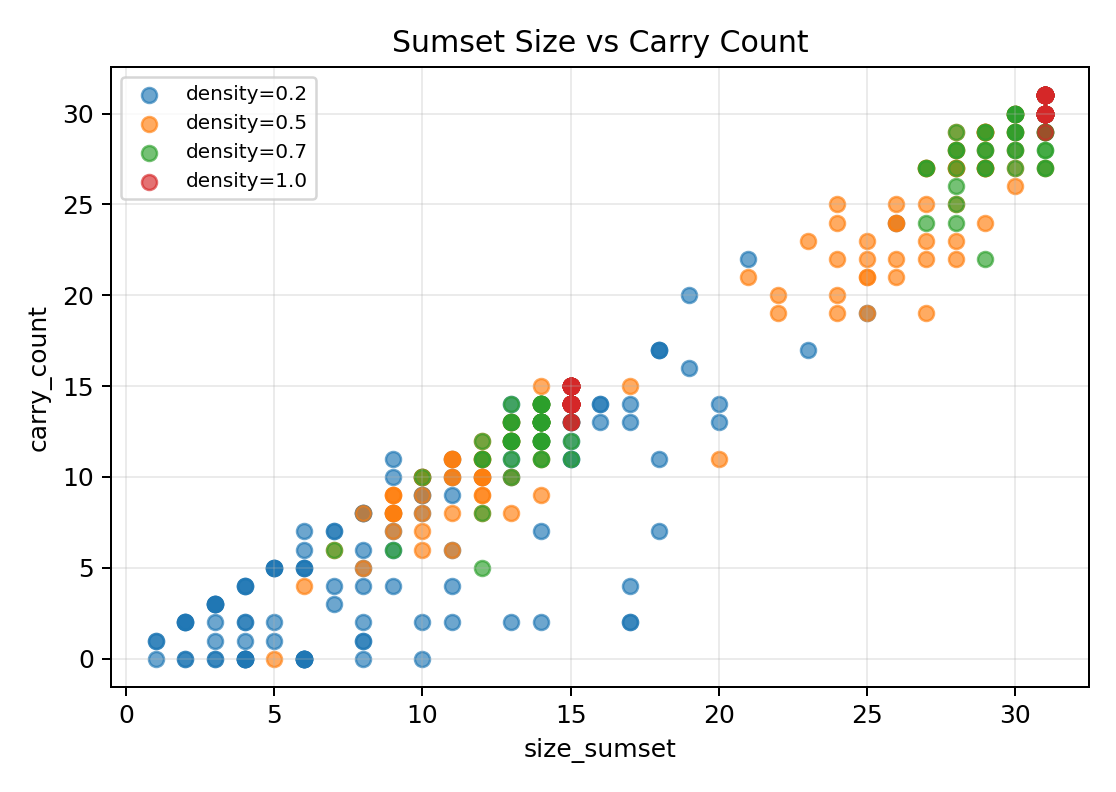
\includegraphics[width=0.78\linewidth]{figures/size_sumset_vs_carry_count.png}
    \caption{Support-sumset size versus carry count.}
    \label{fig:sumset-carry-count}
\end{figure}

\begin{figure}[ht]
    \centering
    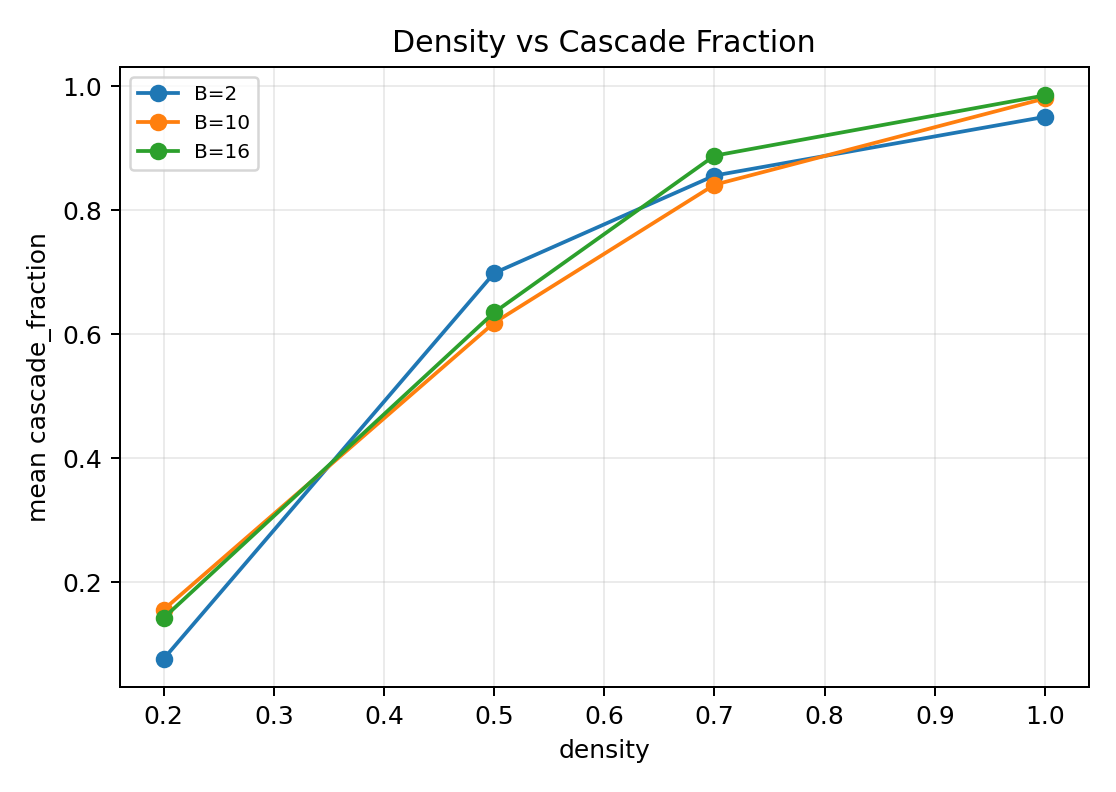
\includegraphics[width=0.78\linewidth]{figures/density_vs_cascade_fraction.png}
    \caption{Support density versus cascade fraction.}
    \label{fig:density-cascade}
\end{figure}

\paragraph{Base effects and normalized metrics.}
Base affects absolute carry mass and normalized amplification differently.
Figure~\ref{fig:base-amplification} shows carry amplification by base, while
Figure~\ref{fig:base-carry-mass-per-digit} shows carry mass per digit. Larger
bases raise the local activation threshold but also allow larger digit
products. The normalized plots should therefore be read together with the raw
plots rather than as replacements.

\begin{figure}[ht]
    \centering
    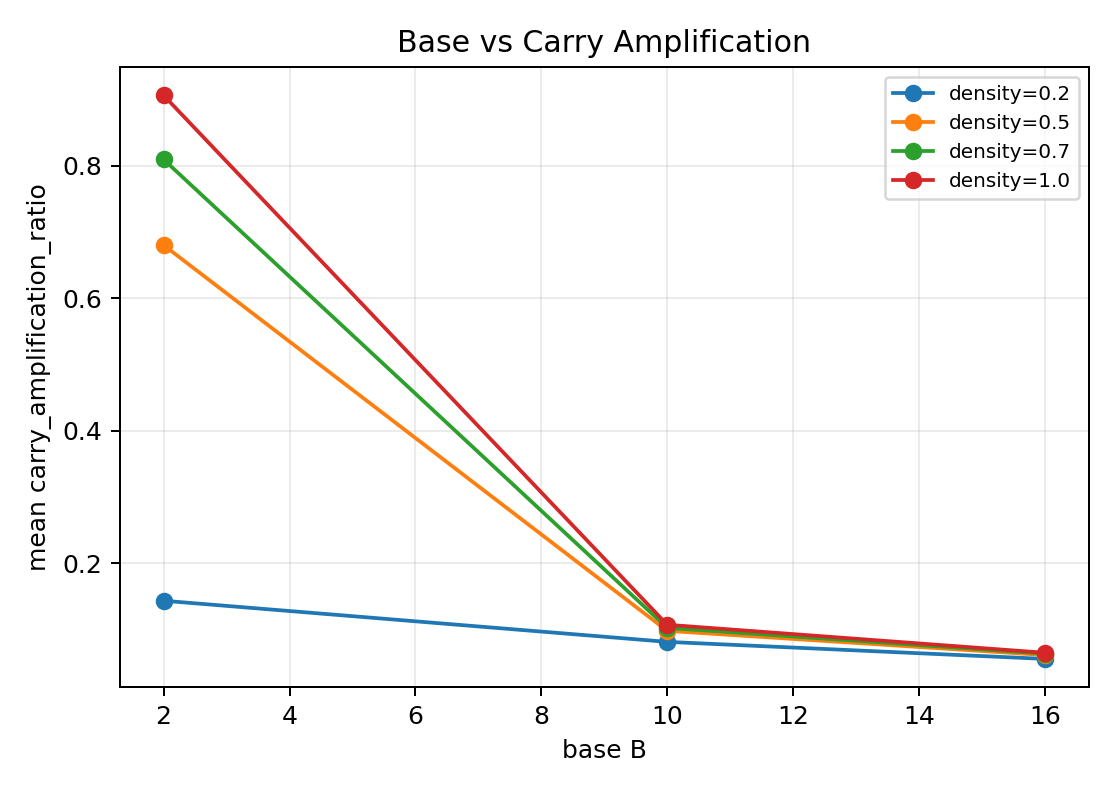
\includegraphics[width=0.78\linewidth]{figures/base_vs_carry_amplification.png}
    \caption{Base versus carry amplification ratio.}
    \label{fig:base-amplification}
\end{figure}

\begin{figure}[ht]
    \centering
    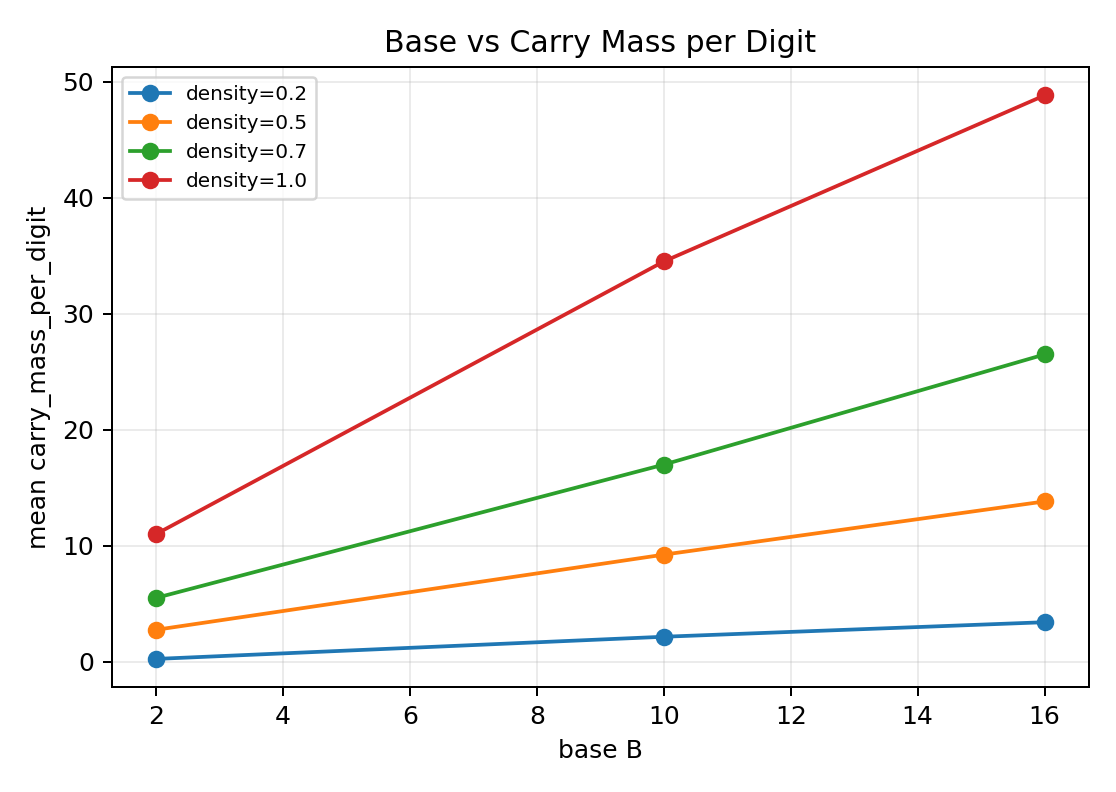
\includegraphics[width=0.78\linewidth]{figures/base_vs_carry_mass_per_digit.png}
    \caption{Base versus carry mass per digit.}
    \label{fig:base-carry-mass-per-digit}
\end{figure}

\paragraph{Interpreting normalization.}
Figure~\ref{fig:normalized-energy} shows normalized additive energy against
carry mass per digit. Normalized additive energy alone is insufficient because
it removes scale: two supports can have similar normalized concentration but
very different total interaction mass. This reinforces the central
interpretation: support geometry gives potential concentration, while digit
amplitudes and incoming carry determine realized carry flow.

\begin{figure}[ht]
    \centering
    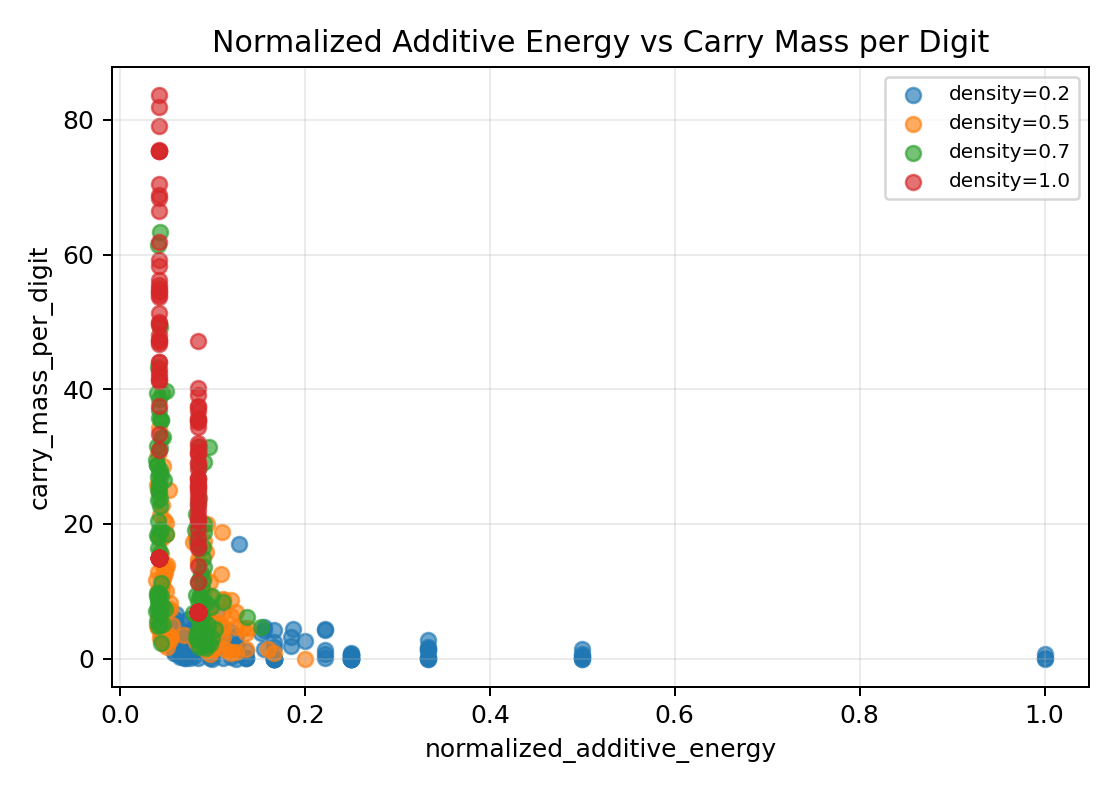
\includegraphics[width=0.78\linewidth]{figures/normalized_additive_energy_vs_carry_mass_per_digit.png}
    \caption{Normalized additive energy versus carry mass per digit.}
    \label{fig:normalized-energy}
\end{figure}
